\chapter{Reservoir Computing}
\label{rc}

\gls{rc} is a bio-inspired artificial \gls{rnn} which is based on the \gls{esn} introduced by Herbert Jaeger in \cite{Jaeger2004}. This computation scheme is well suited for real-time data processing and for chaotic time series prediction\cite{Jaeger2004, JaegerH.2001Tesa, Lukoeviius2012}, and achieves state of the art performances in those domains, as well as in speech recognition\cite{Verstraeten2006, NIPS2010_4056, Jaeger2007}, nonlinear channel equalisation\cite{Jaeger2004} and financial forecasting \cite{financialTimeSeries}.\\

The first section of this chapter introduces the different concepts linked with \rc. It starts by giving a brief overview on the \gls{nn} computation paradigm from which \rc has been derived. After that, the structure, operating principles and features of \rcer are presented. Then, a few elements of \gls{ml} are mentioned in order to have a first glimpse of the training procedure for \rcer. The second section is devoted to the mathematical model governing a \rcer. The last section is about Photonic Reservoir Computers. During the last decade, several physical implementations of \rcer have been proposed, some of which being optical setups. This kind of \rcer is presented, and most specifically reservoir involving \gls{tdm}. Finally, a \rcer is used to resolve two different benchmark tasks and the results on the computations are shown.

\section{Reservoir Computing framework}

%%% ARTIFICIAL NEURAL NETWORK %%%

\subsection{Artificial Neural Network}

A \gls{rcer} is specific kind of \gls{nn}, which is a computation paradigm mimicking the behaviour of a biological brain. The artificial neurons are simply interconnected entities carrying an activation level. The way the activation level is updated depends on the scheme, but the basic idea is common for all of them: a neuron receives a linear combination of the activation level of the neurons to which it is connected, and then computes a nonlinear transformation of this value. This gives the new activation level. On figure \ref{nn}, a feedforward \gls{nn} is depicted. It is called feedforward because the computation goes from left (input neurons in red) to right (output neurons in green). Feedforward \gls{nn} are organised in layers, and a neuron from one layer can only be influenced by neurons in the adjacent layers. This is shown on the Figure by the arrows representing the connections. The gray neurons in the middle belong to the hidden layers, which are used to improve the computing power of such networks. The results of a computation can be read on the activation level of the output neurons \cite[p.727]{russell2010artificial}\cite[p.225]{bishop2006pattern}.

\begin{figure}[h]
	\centering
	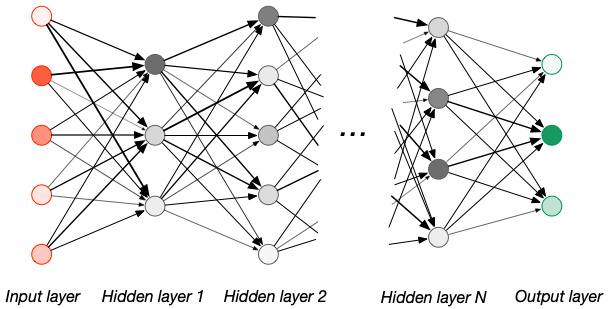
\includegraphics[width=.6\textwidth]{nn}
	\caption{Schematic representation of a feedforward \gls{nn}.}
	\label{nn}
\end{figure}

%%% RESERVOIR COMPUTING %%%

\subsection{Reservoir Computing}

\rcer have been designed to process time dependent inputs, so their structure is inherently different from that of a feedforward \gls{nn}, because they need to exhibit other properties. In this scheme, all the neurons are interconnected and form what is called a reservoir. The reservoir is fed with the time dependent input signal it should process. When the reservoir is properly set up, the activation level of each of the neurons becomes a systematic transformed version of the input signal \cite{Jaeger2004}. This operating point is called the echo state and allows \rcer to reach their best performances \cite{Goudarzi2014ACS, JaegerH.2001Tesa}. In this regime, \rcer exhibit a short-term memory of the previous inputs \cite{Jaeger2004}, which could explain why they perform so well in time dependent situations. There are many physical implementations of \rcer proposed in the literature, many of which are based on optical setups \cite{VanderSande2017}, that is why section \ref{prc} is devoted to them.\\

On figure \ref{rc_principle}, a \rcer is shown. The neurons of the reservoir are represented in orange. They characterise what is called the state of the reservoir, which is encoded by $\mathbf{x}(t)$. They are coupled by the connection matrix $\mathbf{W}$. The input signal $u(t)$ is fed into the input neuron (blue) and is coupled to the reservoir \textit{via} the input matrix $\mathbf{W}^{\text{in}}$. The output $y(t)$ is read on the output neuron (red) and is obtained thanks to the output matrix $\mathbf{W}^{\text{out}}$. This matrix is the only one that needs to be updated when the reservoir is learning. This task is not straightforward, that is why the next paragraph takes care of introducing the different approaches that can be followed to compute $\mathbf{W}^{\text{out}}$. For some applications, it can be useful to also have a feedback of the output sent back into the reservoir. This can be achieved by the feedback matrix $\mathbf{W}^{\text{fb}}$. The mathematical aspects mentioned in this paragraph are detailed in section \ref{rc-mathematical-model}.

\begin{figure}[h]
	\centering
	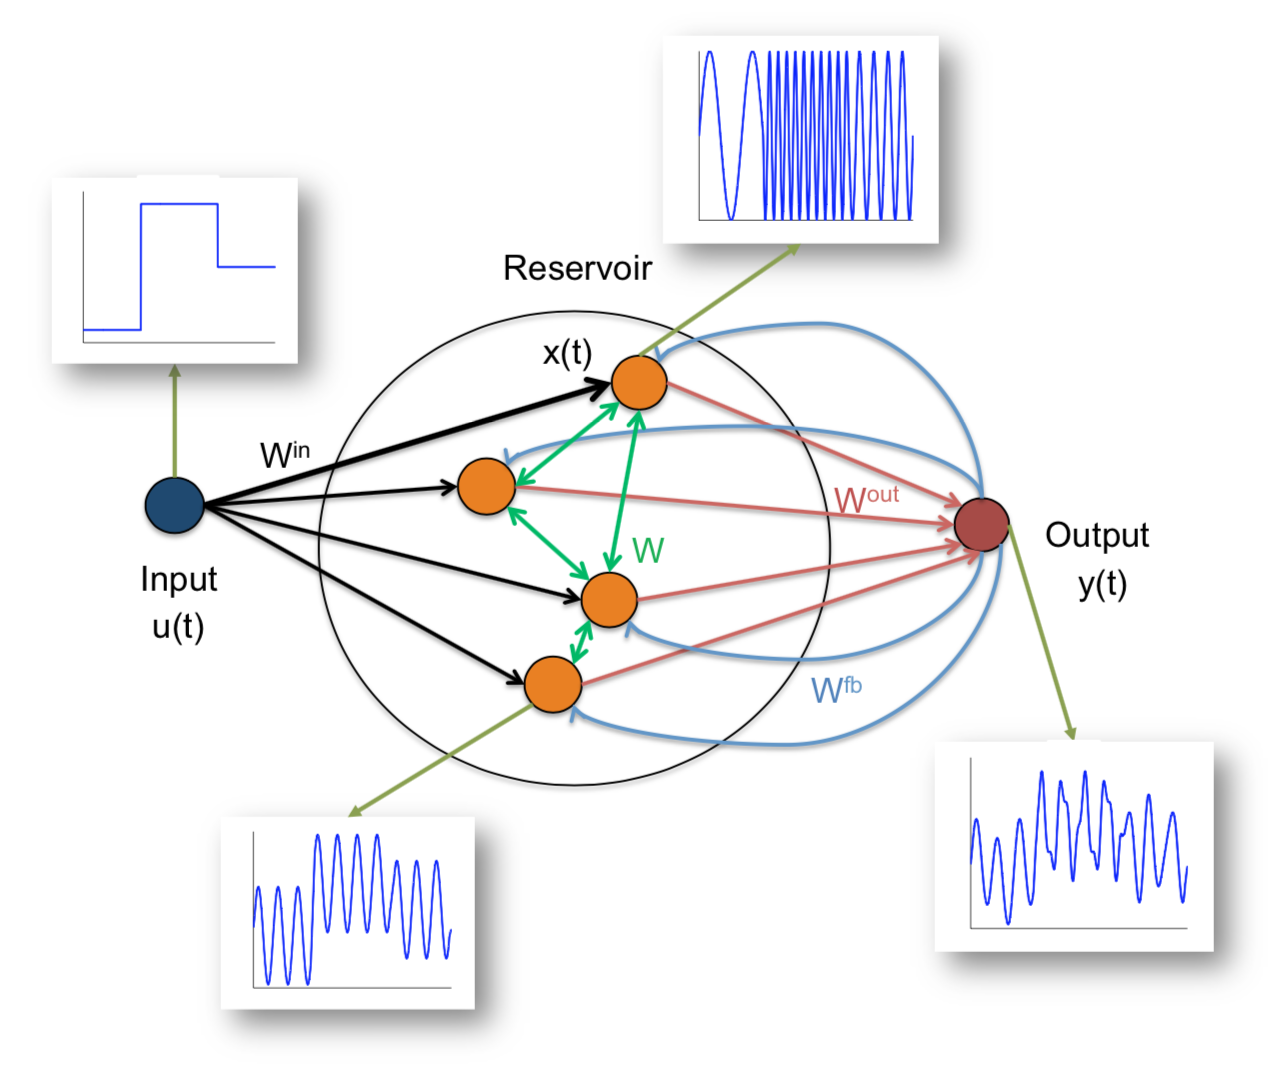
\includegraphics[width=.6\textwidth]{rc_principle.png}
	\caption{Schematic representation of a \acrlong{rcer} \cite{financialTimeSeries}.}
	\label{rc_principle}
\end{figure}

%%% MACHINE LEARNING %%%

\subsection{Machine Learning}

Regardless of the learning scheme used to train a \gls{nn}, the basic idea is always to minimise the difference between the desired and the actual outputs. In practice, this is achieved by updating the different connection coefficients of the \gls{nn} \cite[p.233]{bishop2006pattern}\cite[p.733]{russell2010artificial}. This procedure often turns out to be a really complicated task for feedforward \gls{nn}, which explains why the development of efficient \gls{ml} algorithms is such a hot topic nowadays. In contrast, as can be seen on figure \ref{rc-ml}, \gls{rcer} only need their output weights to be adjusted when being trained, which makes them computationally lighter \cite{Jaeger2004}. This is due to the fact that the connections of the reservoir should not contain any information about the task, but should only be used to reach the \gls{esn} regime, as mentioned in the previous paragraph. There are two main families of training methods for \gls{rcer} \cite{Jaeger2002}. On the one hand, there is the \textit{batch learning}, which comprises the methods requiring to first store a wealth of data regarding the task being taught before being able to actually compute the output weights. Once enough data is gathered, this kind of algorithms returns the optimal weights all at once. They present the advantage of involving only one training phase, after which the \gls{rcer} are ready to perform. However, the need for vast amount of data and the inability for the \gls{rcer} to adapt to an input evolving out of the range for which it has been trained are two drawbacks. On the other hand, \textit{online learning} methods allow to iteratively improve the output weights. Therefore, starting from a first guess, these algorithms can converge to suitable output weights. They are much more adaptable than the batch learning ones. However, their convergence is not guaranteed and can be slow \cite{JaegerTraining, schrauwen}.

\begin{figure}[h]
	\centering
	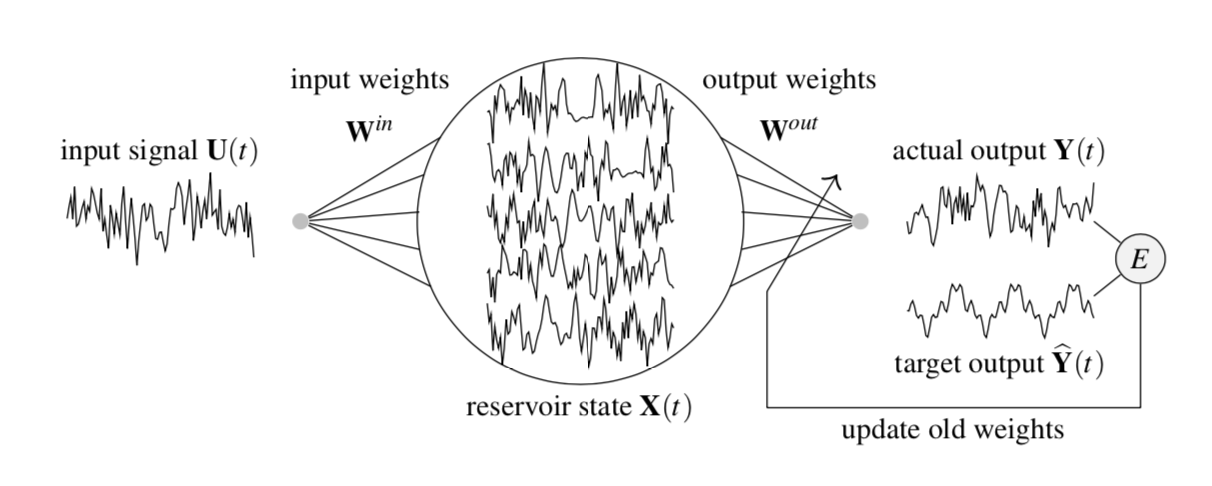
\includegraphics[width=.7\textwidth]{rc-ml.png}
	\caption{Learning procedure for \acrlong{rcer} \cite{Goudarzi2014ACS}.}
	\label{rc-ml}
\end{figure}

%%%%%%%%% MATHEMATICAL MODEL %%%%%%%%%%

\section{Mathematical Model}

\label{rc-mathematical-model}

In this section, an overview of the mathematical framework is given. First, the different objects are formally defined, and their dynamics is presented. Then, a few key elements about the computation of the output weights are introduced.

%%% DYNAMICS OF THE RESERVOIR %%%

\subsection{Dynamics of the reservoir}

let us define the \textit{state} of the reservoir. As said previously, the \gls{rc} can be fully described by the activation level of each of its neurons. The state is therefore defined as a vector whose components are the activation levels of the neurons. If the number of neurons making up the reservoir is $N$, and if $x_i$ is the activation level of the $i^{\text{th}}$ neuron, then the state vector reads as follows:

\begin{equation}
	\mathbf{x} = \begin{bmatrix}
		x_1\\
		\vdots \\
		x_i \\
		\vdots \\
		x_N
	\end{bmatrix}
\end{equation}

The dynamics governing the state vector and the output of the reservoir proposed in \cite{JaegerH.2001Tesa} are presented below. In practice, it is too general for the implementations studied in this work. However, the equations are introduced without loss of generality, and simplifying assumptions applying the photonic implementations of \rcer will be specified in the section devoted to them.

\begin{align}
	\mathbf{x}(n+1) &= \mathbf{f} \left( \mathbf{W}^{\text{in}} \mathbf{u}(n+1) + \mathbf{W} \mathbf{x}(n) + \mathbf{W}^{\text{fb}} \mathbf{y}(n) \right) \label{rc_dynamics}\\
	\mathbf{y}(n+1) &= \mathbf{f}^{\text{out}} \left( \mathbf{W}^{\text{out}} \left(\mathbf{x}(n+1), \mathbf{u}(n+1), \mathbf{y}(n)\right) \right) \label{rc_output}
\end{align}

Different elements need to be defined: 

\begin{itemize}
	\item $n \in \{1, \dots, T\}$ is the discrete time variable
	\item $\mathbf{u} \in \mathbb{C}^k$ is the input vector which enters the reservoir through the input neurons
	\item $\mathbf{W}^{\text{in}} \in \mathbb{C}^{N \times k}$ is the input matrix. It indicates how the $k$ input neurons are connected to the neurons of the reservoir
	\item $\mathbf{x} \in \mathbb{C}^{N}$ is the state vector, as said previously
	\item $\mathbf{W} \in \mathbb{C}^{N \times N}$ is the synaptic matrix, or the connection matrix which has already been introduced
	\item $\mathbf{y} \in \mathbb{C}^{m}$ is the output vector of the reservoir whose value can be read out on the output neurons
	\item $\mathbf{W}^{\text{fb}} \in \mathbb{C}^{N \times m}$ is the feedback matrix. It couples the output back into the reservoir
	\item $\mathbf{f}: \mathbb{C}^N \mapsto \mathbb{C}^N$ is the nonlinear function mapping the linear combination it receives as argument to a valid state vector
	\item $\left(\mathbf{x}(n+1), \mathbf{u}(n+1), \mathbf{y}(n)\right)$ is the concatenation of those three vectors
	\item $\mathbf{W}^{\text{out}} \in \mathbb{C}^{m \times (N+k+m)}$ is the output matrix of the reservoir. It is optimised through \gls{ml}
	\item $\mathbf{f}^{\text{out}} : \mathbb{C}^{m} \mapsto \mathbb{C}^{m}$ is the output function of the reservoir
\end{itemize}

%%% COMPUTATION OF THE OUTPUT WEIGHTS %%%

\subsection{Computation of the output weights}

\label{subsec-rc-training}

To determine the output matrix $\mathbf{W}^{\text{out}}$ in the batch learning approach, one needs to perform a ridge (or Tikhonov) regression \cite{NIPS2010_4056}, which is an improved version of multivariate linear regression that improves the numerical stability of the scheme, and that prevents overfitting of the data. By restricting the desired output to a scalar function $\hat{y}(n)$ and by taking a learning period of $T$ time steps, one defines the matrices $\mathbf{X}$ and $\hat{\mathbf{Y}}$ and solves the following equation to find the output weights vector $\mathbf{W}^{\text{out}}$:

\begin{equation}
	\mathbf{X} = \begin{bmatrix}
			x_0(0) & x_1(0) & \dots & x_N(0)\\
			x_0(1) & x_1(1) & \dots & x_N(1)\\
			\vdots & & & \vdots \\
			x_0(T) & x_1(T) & \dots & x_N(T)			
	\end{bmatrix},~ \hat{\mathbf{Y}} = \begin{bmatrix}
		\hat{y}(0)\\
		\hat{y}(1)\\
		\vdots \\
		\hat{y}(T)
	\end{bmatrix}
\end{equation} 

\begin{equation}
	\left(\mathbf{X}^{\text{T}} \mathbf{X}+\epsilon \mathbf{I} \right) \mathbf{W}^{\text{out}} = \mathbf{X}^{\text{T}} \hat{\mathbf{Y}}
	\label{ridge-regression}
\end{equation}

Here $\epsilon$ is the constant used for the Tikhonov regression. By setting $\epsilon$ to 0, one finds the \textit{normal equation} that comes up when solving a linear regression \cite{Goudarzi2014ACS} in the sense of the least squares. This procedure can be generalised to higher dimensions desired output vectors $\hat{\mathbf{y}}(n)$. Different optimisation algorithms can be used to compute the output weights in practice, but their description is out of the scope of this work, see \cite{Lukoeviius2009} for more details.\\

Different metrics can be used to capture the distance between the actual and the desired outputs. In the literature, one of the most frequent ones is the \gls{nmse} \cite{Duport2016} (with $\hat{\mathbf{y}}(n)$ the target vector, $\langle \dots \rangle _n$ the average with respect to $n$, and $\| \dots \|$ the euclidean norm):

\begin{equation}
	\text{NMSE} = \frac{\langle \| \hat{\mathbf{y}}(n) - \mathbf{y}(n)\|^2 \rangle _n}{\langle \| \hat{\mathbf{y}}(n) - \langle \hat{\mathbf{y}}(n) \rangle _n \|^2 \rangle _n}
\end{equation}

%%%%%%%%%% INTRODUCTION TO PHOTONIC RESERVOIR COMPUTING %%%%%%%%%%

\section{Introduction to Photonic Reservoir Computing}

\label{prc}

As already mentioned, different implementations of \gls{prc} have been proposed \cite{VanderSande2017}. In this section, systems in which neurons are multiplexed in time are studied because they constitute a good first approach to \gls{prc} and because they bring insights that are interesting for the scheme explored in this thesis. However, it is worth mentioning that one can find among others spatially distributed \rcer based on fully integrated silicon-chip with nonlinearities stemming from \acrlongpl{soa} \cite{Vandoorne2014}, and on diffractively coupled Vertical-Cavity Surface-Emitting Lasers \cite{Brunner2015}. \\

In this section, the assumptions applying to reservoir with \gls{tdm} of the neurons are first presented. Indeed, the equations introduced in the previous section can be substantially simplified when one is working with this kind of reservoir. After that, setups where neurons are encoded in the intensity of the light are considered. Finally, experiments in which the neurons are represented in the phaser of the electric field are presented. Recalling that the light intensity is proportional to the squared modulus of the phaser of the electric field, it is shown that the outputs of these two kinds of reservoir are different, but analogous, and that they rely on the same mathematical interpretation. The latter scheme is studied with greater length since it reaches state of the art performances in classical benchmark tasks and since the novel implementation which is the main topic of this work shares some features with it. As a last remark, and to give a better understanding on the flexibility of \rcer, in \cite{Fernando2003} the researchers managed to perform speech recognition and to resolve the XOR problem\footnote{The XOR task consists in reproducing the behaviour of a logical XOR gate, which is a task of historical importance for \gls{nn} \cite{minsky1969perceptrons}.} in a bucket of water.\\

%%% TDM OF THE NEURONS %%%

\subsection{Time Division Multiplexing of the neurons}

\label{tdm-neurons}

 Many implementations of \rcer based on \gls{tdm} of the neurons have been proposed in the literature \cite{Paquot2012, Antonik2017, Duport2016, Dejonckheere2014, Vandoorne2008, Vinckier2015}. Let $T$ be the time scale of the input signal. It should be close to the \gls{rtt} of the delay line, but not  exactly the same in order to be able to couple the neurons. The detuning between the \gls{rtt} and $T$ is controlled by the integer parameter $k$. On figure \ref{tdm-neurons-principle}, one can observe how the neurons can be multiplexed in time. One can see that the allocated window for each of the neurons lasts $\theta = T/N$. Since $\theta$ cannot be arbitrarily small in practice\footnote{If $\theta$ gets too short, it exceeds the bandwidth of measurement devices, so it becomes impossible to measure the neurons.}, this implies that the greater the number of neurons, the greater $T$ and thus the slower the time scale of the input data. This suggests that one should look for a tradeoff between accuracy and speed in data processing for this kind of \rcer. For example, in \cite{Vinckier2015}, the refresh rate of the input is around 0.9 GHz.
 
 \begin{figure}[h]
 	\centering
 	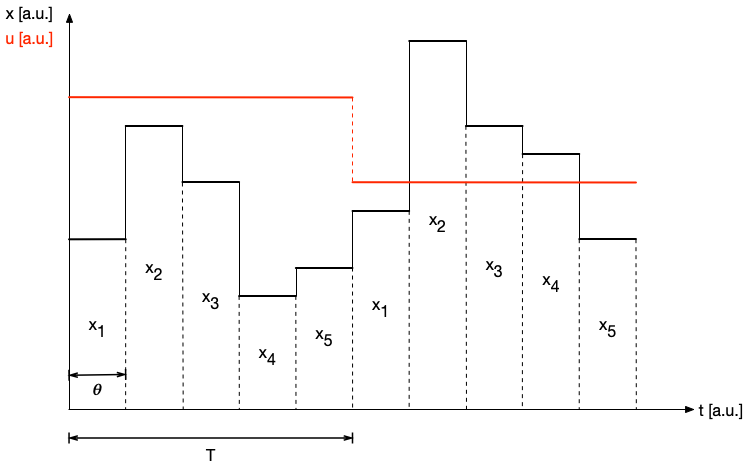
\includegraphics[width=.8\textwidth]{tdm-neurons-principle}
 	\caption{Schematic representation of the evolution of the neurons in time for a \gls{tdm} reservoir.}
 	\label{tdm-neurons-principle}
 \end{figure}
 

%%% SIMPLIFYING ASSUMPTIONS %%%

\subsection{Simplifying assumptions}

In this section, the mathematical framework introduced in section \ref{rc-mathematical-model} is adapted to describe the behaviour of \gls{tdm} \gls{prc} in a suitable way. Further details concerning specific types of \gls{prc} are added in the following sections which are devoted to them.

\paragraph{Input and connection matrices}

The input of the reservoir is real scalar function $u(n)$ for \gls{prc}, therefore the expression of $\win$ becomes a real vector of length $N$ which is called the \textit{input mask} $\mathbf{m}$ in the literature. The input mask can be chosen in different ways: in \cite{Duport2016}, they use a sinusoidal input mask whereas in \cite{Antonik2017, Vinckier2015, Paquot2012} the input masks are randomly chosen.\\

Very few constraints apply to the creation of the connection matrix $\w$. It can be randomly generated and sparse. However, to make the occurence of the echo state more likely to happen, one wants to work with a spectral radius $\rho \left( \w \right)<1$. If this condition is not verified, as well as degrading the performance of the reservoir, this can also lead to instabilities \cite{Lukoeviius2009}.\\

The matrices $\w$ and $\win$ can be rescaled, and this scaling can alter the performances of the reservoir. One should therefore design the \gls{prc} in such a way that those scaling factors are easily accessible experimentally. If one defines $\alpha$ and $\beta$, the feedback\footnote{This may seem like a misnomer at this point since it has nothing to do with $\wfb$, but this name is used because $\alpha$ acts as a gain for the activation level of the neurons being fed back into the reservoir.} and input gains, the input and connection matrices become:

\begin{equation}
	\w \longrightarrow \alpha \mathbf{A}, \quad \win \longrightarrow \beta \mathbf{m}
\end{equation}

\paragraph{Feedback and output}

The output signal of a \gls{prc} is a real scalar function $y(n)$, which means that the output matrix $\wout$ becomes a real vector. Furthermore, the concatenation of $\mathbf{x}(n+1), \mathbf{u}(n+1), y(n)$ appearing in equation \eqref{rc_output} is not used, but only the state vector $\mathbf{x}$, hence the fact that $\wout$ is of dimension $N$. Regarding the feedback of the output into the reservoir, it is currently not doable in practice. This is due to the fact that, when running a \rc experiment, some post-processing of the data needs to be performed on a computer in order to obtain the output.\\

With all these simplifications, equations \eqref{rc_dynamics} and \eqref{rc_output} reduce to:

\begin{align}
	\mathbf{x}(n+1) &= \mathbf{f} \left( \alpha \mathbf{A} \mathbf{x}(n) + \beta \mathbf{m} u(n+1) \right)\\
	y(n+1) &= f^{\text{out}} \left( \mathbf{W}^{\text{out}} \mathbf{x}(n+1) \right)
\end{align}

%%% NEURONS ENCODED IN LIGHT INTENSITY %%%

\subsection{Neurons encoded in light intensity}

There are two major families of \gls{tdm} \gls{prc}. The first kind of \gls{prc} are those using optical components exhibiting nonlinear behaviour, such as \gls{mzm} \cite{Duport2016, Paquot2012, Antonik2017}, \gls{soa} \cite{Vandoorne2008} or semiconductor saturable absorber mirror \cite{Dejonckheere2014} to couple the neurons. In an actual optical experiment, the measurements have to be done with photodiodes. These devices can only inform about the intensity of the light, which is the squared modulus of the phaser representation of the electric field, and not about the actual electric field. However, in the scheme presented above, the input and the activation level of the neurons are real valued functions appropriately encoded in the intensity of the light, and can therefore be directly read out by a photodiode, hence this simple expression for the output of the reservoir:

\begin{equation}
	y(n+1) = \sum_{i=1}^{N} W^{\text{out}}_i x_i (n+1) = (\wout)^{\text{T}} \cdot \mathbf{x}(n+1)
	\label{lin_output_rc}
\end{equation}

%%% NEURONS ENCODED IN COMPLEX ELECTRIC FIELD %%%

\subsection{Neurons encoded in phaser representation of the electric field}

\label{rc-lin-complex}

On the other hand, in \cite{Vinckier2015}, coherent light is used and the neurons are encoded in the complex phaser representation of the electric field and are linearly coupled using a delay line. In this scheme, the reservoir is linear, as can be seen on equation \eqref{rc_lin_dynamics}. This kind of \rcer is described with greater length because the new approach studied in this thesis relies on on a linear reservoir as well. In this equation, $\alpha$ and $\beta$ are the feedback and input gains, respectively, $A_0$ is the input bias, $\phi$ is the phase acquired by the electric field during by going through the delay line, and $k$ is the detuning parameter.

\begin{equation}
	x_i(n+1) = 
	\begin{cases}
		\alpha e^{j\phi} x_{i-k}(n)+\beta \left(m_i u(n) +A_0 \right) & \text{if } k \leq i \leq N\\
		\alpha e^{j\phi} x_{N+i-k}(n-1)+\beta \left(m_i u(n) +A_0 \right) & \text{if } 0 \leq i \leq k			
	\end{cases}
	\label{rc_lin_dynamics}
\end{equation}

The equation can be rewritten in a compact way:

\begin{equation}
	\mathbf{x}(n+1) = \alpha \mathbf{A} \mathbf{x}(n) + \beta (\mathbf{m} u(n+1)+ \mathbf{A_0})
	\label{rc_lin_dynamics}
\end{equation}

It thus appears more clearly why the condition mentioned previously regarding $\rho \left( \alpha \mathbf{A} \right)$ is relevant. Indeed, by neglecting the inputs, if $\mathbf{x}_j$ is an eigenvector of $\alpha \mathbf{A}$ with eigenvalue $\lambda_j>1$, the above equation will lead to an exponential divergence $\mathbf{x}_j(n) \sim \lambda_j^n \mathbf{x}_j(0)$. On the other hand, if $\lambda_j$ is too small, the state $\mathbf{x}_j$ will be damped too quickly, deteriorating the short-term memory capabilities of the reservoir and preventing it from reaching the echo state. \\

In the linear reservoir, since the neurons and the input are inscribed in the complex electric field, the nonlinearity is introduced by the read out photodiodes. The output is therefore given by:

\begin{equation}
	y(n+1) = \sum_{i=1}^{N} W^{\text{out}}_i |x_i (n+1)|^2
	\label{quad_output_rc}
\end{equation}

From a historical point of view, it is interesting to notice that this reservoir shares features with the first artificial \gls{nn}, the \emph{perceptron}, introduced by F. Rosenblatt in 1958 \cite{Rosenblatt58theperceptron}, which also had a linear connection matrix, and a nonlinear output function.\\

 Equations \eqref{lin_output_rc} and \eqref{quad_output_rc} give an interesting intuition on the meaning of the \gls{esn}. Indeed, as said previously, when a \rc reaches the echo state, each of the neurons tends to systematically reproduce a modified version of the input, the actual modification being an individual characteristic of each neuron \cite{Jaeger2004}. One can see this feature in the perspective of linear algebra. When the \rcer is fed with an input, it creates a set of time varying functions that can be seen as a basis in which one can try to express the output of the reservoir, which is a vector in the vectorial space of functions. This is why it is often said in the literature that a \rcer maps an input to a higher dimensional space. Therefore, one can in theory approach any target function with an arbitrary precision, depending on the number of neurons in the reservoir \cite{Jaeger2004}. The higher the number of neurons, the closer to a genuine series development one gets.\\

%%% SIMULATIONS %%%

\subsection{Simulations}

In this section, the performance of the linear reservoir with quadratic output from \cite{Vinckier2015} are estimated with simulations. Two benchmark task are tackled, first \acrshort{narma}10 and then nonlinear channel equalisation.

% NARMA10 %

\subsubsection{\acrshort{narma}10}

\gls{narma}  10 is a model often used to simulate chaotic time series because it exhibits similar properties \cite{Paquot2012}. If $u(n)$ is a random variable uniformly distributed along the interval $[-0.5, 0.5]$, the recurrent equation for \gls{narma}10 reads:

\begin{equation}
	\hat{y}(n+1) = 0.3\hat{y}(n)+0.05\hat{y}(n)\left(\sum_{i=0}^9 \hat{y}(n-i) \right)+1.5u(n-9)u(n)+0.1
\end{equation}

\begin{figure}[h]
	\centering
	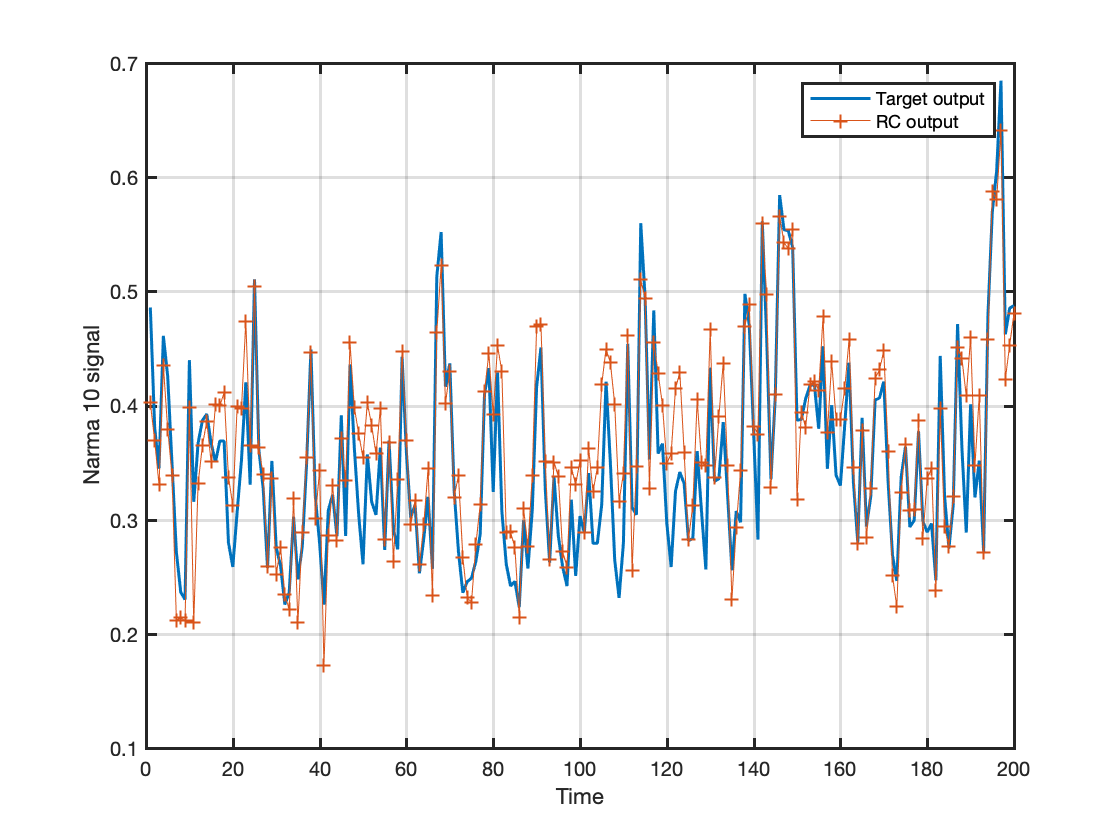
\includegraphics[width=\textwidth]{narma10.png}
	\caption{\gls{narma}10 task with \gls{nmse} equal to 0.1541. This reservoir is made of 50 neurons. $\alpha=0.5$, $k=7$, $\phi=0$ rad, $\beta=1$, $A_0=1$, $\mathbf{m}$ is a random vector distributed between 0 and 1. The first 300 time steps were discarded in order to let enough time to the reservoir to enter the echo state (washout). Then the reservoir was trained for 3000 time steps and tested over 6000 time steps. This reservoir is particularly well suited for  \gls{narma}10 since the nonlinearities in the signal are mostly quadratic.}
	\label{narma10}
\end{figure}

% NONLINEAR CHANNEL EQUALISATION %

\subsubsection{Nonlinear channel equalisation}

This task consists in the reconstruction of a signal after it has travelled through a nonlinear channel. The emitted signal $\hat{y}$ is randomly drawn from the symbol set $\{-3,-1,1,3\}$. It is first superposed with following and preceding symbols as can be seen in \eqref{signal_mixing}. After that, a third degree polynomial transformation is applied to the mixed signals, and a Gaussian noise, whose intensity can be set in order to adjust the signal to noise ratio, is added in \eqref{nonlinear_ch}. This metric used to evaluate the performance of the reservoir for this type of task is the \gls{ser} and is defined as the ratio between the number of erroneous symbols and the total number of symbols.

\begin{align}
	q(n) &= 0.08\hat{y}(n+2)-0.12\hat{y}(n+1)+\hat{y}(n)+0.18\hat{y}(n-1) \nonumber\\
	&-0.1\hat{y}(n-2)+0.091\hat{y}(n-3)-0.05\hat{y}(n-4) \nonumber\\
	&+0.04\hat{y}(n-5)+0.03\hat{y}(n-6)+0.01\hat{y}(n-7) \label{signal_mixing}
\end{align}

\begin{equation}
	u(n)=q(n)+0.036q(n)^2-0.011q(n)^3+\nu(n)
	\label{nonlinear_ch}
\end{equation}

\begin{figure}[h]
	\centering
	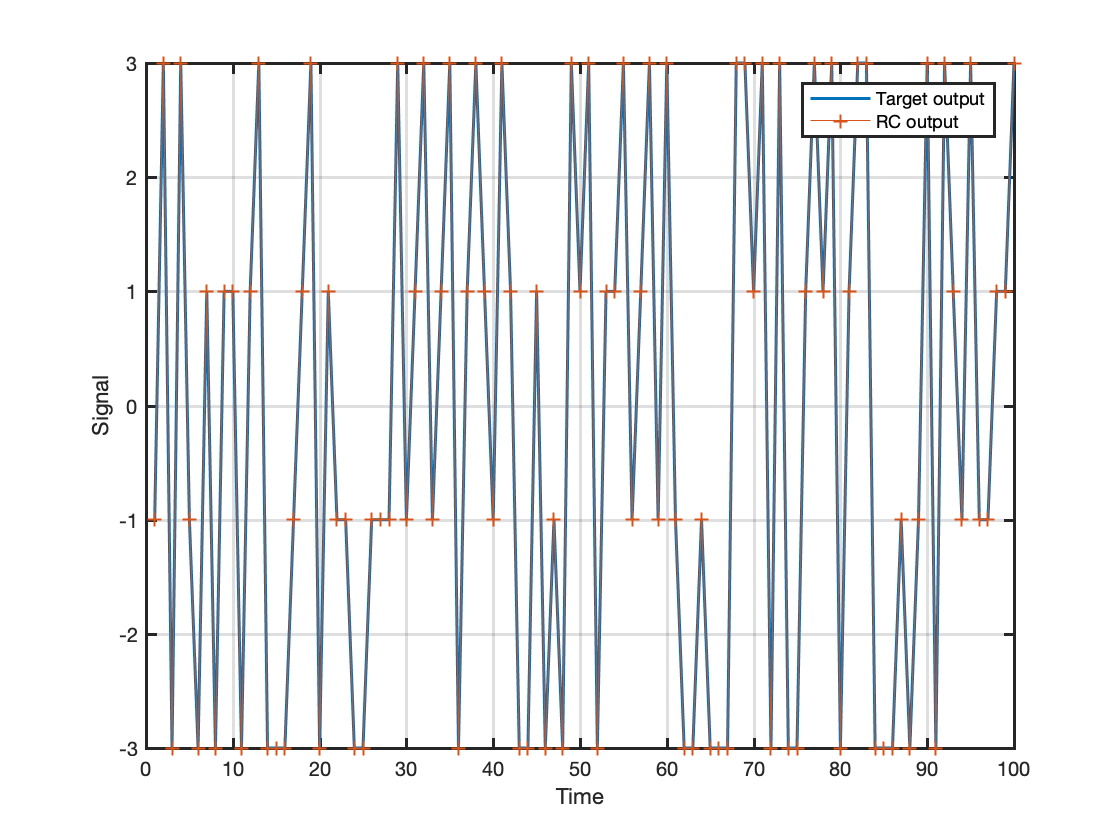
\includegraphics[width=\textwidth]{nonlinear_ch_eq}
	\caption{Nonlinear channel equalisation task with a signal error rate of $5~10^{-4}$, with \gls{snr} equal to 32 dB. This reservoir is made of 50 neurons. $\alpha=0.5$, $k=7$, $\phi=0$ rad, $\beta=1$, $A_0=1$, $\mathbf{m}$ is a random vector distributed between 0 and 1. The first 300 time steps were discarded in order to let enough time to the reservoir to enter the echo state (washout). Then the reservoir was trained for 3000 time steps and tested over 6000 time steps. The symbols predicted by the \rcer are found by changing the continuous valued output by the closest symbol.}
\end{figure}
